\documentclass[12pt,a4paper]{article}

% ─── Page Layout ───────────────────────────────────────────────────────────────
\usepackage[a4paper, margin=0.8in, headheight=14pt]{geometry}

% ─── Fonts (XeLaTeX) ───────────────────────────────────────────────────────────
\usepackage{fontspec}
\usepackage{unicode-math}
\setmainfont{TeX Gyre Pagella}
\setmonofont[Scale=0.88]{TeX Gyre Cursor}
\setmathfont{Latin Modern Math}

% ─── Packages ──────────────────────────────────────────────────────────────────
\usepackage{xcolor}
\usepackage{colortbl}
\usepackage{titlesec}
\usepackage{enumitem}
\usepackage{tabularx}
\usepackage{booktabs}
\usepackage{array}
\usepackage{amsmath}
\usepackage{tikz}
\usetikzlibrary{shapes.geometric, arrows.meta, positioning, calc, fit, decorations.pathreplacing}
\usepackage{tcolorbox}
\tcbuselibrary{skins, breakable}
\usepackage{hyperref}
\usepackage{fancyhdr}
\usepackage{graphicx}
\usepackage{microtype}
\hyphenpenalty=10000
\exhyphenpenalty=10000
\sloppy
\usepackage{caption}
\usepackage{setspace}
\usepackage{multirow}
\usepackage{tocloft}

% ─── Q&A helper ────────────────────────────────────────────────────────────────
\newcommand{\Q}[1]{\textbf{#1}\par\noindent\ignorespaces}

% ─── Colour Palette ────────────────────────────────────────────────────────────
\definecolor{myred}{RGB}{196,30,58}
\definecolor{mydark}{RGB}{30,30,50}
\definecolor{mygreen}{RGB}{14,120,80}
\definecolor{myteal}{RGB}{0,130,140}
\definecolor{myamber}{RGB}{180,100,0}
\definecolor{mypurple}{RGB}{100,30,160}
\definecolor{mygray}{RGB}{246,247,249}
\definecolor{mgframe}{RGB}{180,185,200}
\definecolor{watermark}{RGB}{145,150,170}
\definecolor{hdrred}{RGB}{250,232,235}
\definecolor{hdrgreen}{RGB}{220,244,233}
\definecolor{hdrteal}{RGB}{220,242,244}
\definecolor{hdramber}{RGB}{253,242,215}
\definecolor{hdrpurple}{RGB}{238,228,255}
\definecolor{hdrgray}{RGB}{238,240,245}
\definecolor{rowalt}{RGB}{250,251,253}

% ─── Section Formatting ────────────────────────────────────────────────────────
\titleformat{\section}
  {\large\bfseries\color{myred}}{\thesection.}{0.5em}{}
  [\vspace{1pt}{\color{myred}\rule{\linewidth}{0.8pt}}]
\titleformat{\subsection}
  {\normalsize\bfseries\color{myteal}}{\thesubsection}{0.5em}{}
\titlespacing*{\section}{0pt}{18pt}{7pt}
\titlespacing*{\subsection}{0pt}{11pt}{4pt}

% ─── Paragraph ─────────────────────────────────────────────────────────────────
\setlength{\parindent}{0pt}
\setlength{\parskip}{4pt}

% ─── TOC Styling ───────────────────────────────────────────────────────────────
\renewcommand{\cfttoctitlefont}{\large\bfseries\color{myred}}
\renewcommand{\cftaftertoctitle}{\par\noindent{\color{myred}\rule{\linewidth}{0.8pt}}}
\setlength{\cftbeforetoctitleskip}{0pt}
\setlength{\cftaftertoctitleskip}{6pt}
\renewcommand{\cftsecfont}{\normalsize\bfseries\color{mydark}}
\renewcommand{\cftsecpagefont}{\normalsize\bfseries\color{mydark}}
\renewcommand{\cftsecleader}{\cftdotfill{\cftdotsep}}
\setlength{\cftbeforesecskip}{7pt}
\renewcommand{\cftsubsecfont}{\small\color{mydark}}
\renewcommand{\cftsubsecpagefont}{\small\color{mydark}}
\setlength{\cftbeforesubsecskip}{3pt}
\setlength{\cftsubsecindent}{1.4em}

% ─── Table helpers ─────────────────────────────────────────────────────────────
\renewcommand{\arraystretch}{1.45}
\setlength{\tabcolsep}{6pt}
\arrayrulecolor{mydark}
\newcolumntype{B}[1]{>{\small\bfseries\raggedright\arraybackslash}m{#1}}
\newcolumntype{Y}{>{\small\raggedright\arraybackslash}X}
\renewcommand{\tabularxcolumn}[1]{m{#1}}

% ─── Header / Footer ───────────────────────────────────────────────────────────
\pagestyle{fancy}
\fancyhf{}
\fancyhead[L]{\small\color{myred}\textbf{OE-EC604A}\;\color{mydark}--- Electronic Measurement \& Instruments}
\fancyhead[R]{\small\color{myteal}\textbf{Module 1 Notes}}
\fancyfoot[C]{\small\color{mydark}\thepage}
\fancyfoot[R]{\small\color{watermark}\textit{\copyright\ Biraj}}
\renewcommand{\headrulewidth}{0.5pt}
\renewcommand{\footrulewidth}{0.3pt}

% ─── Hyperref ──────────────────────────────────────────────────────────────────
\hypersetup{
  colorlinks=true, linkcolor=myteal, urlcolor=myteal,
  pdfauthor={Biraj Sarkar},
  pdftitle={OE-EC604A --- Module 1 Notes}
}

% ─── tcolorbox styles ──────────────────────────────────────────────────────────
\tcbset{
  tikzbox/.style={
    colback=mygray, colframe=mgframe, boxrule=0.6pt, arc=4pt,
    left=8pt, right=8pt, top=6pt, bottom=6pt,
    colbacktitle=mgframe, coltitle=mydark,
    fonttitle=\small\bfseries
  },
  defbox/.style={
    colback=hdrgreen, colframe=mygreen, boxrule=0.8pt, arc=4pt,
    left=9pt, right=9pt, top=6pt, bottom=6pt,
    colbacktitle=mygreen, coltitle=white,
    fonttitle=\small\bfseries
  },
  formulabox/.style={
    colback=hdrteal, colframe=myteal, boxrule=0.8pt, arc=4pt,
    left=9pt, right=9pt, top=7pt, bottom=7pt,
    colbacktitle=myteal, coltitle=white,
    fonttitle=\small\bfseries
  },
  examplebox/.style={
    colback=hdramber, colframe=myamber, boxrule=0.8pt, arc=4pt,
    left=9pt, right=9pt, top=6pt, bottom=6pt,
    colbacktitle=myamber, coltitle=white,
    fonttitle=\small\bfseries
  },
  masonbox/.style={
    colback=hdrpurple, colframe=mypurple, boxrule=0.8pt, arc=4pt,
    left=9pt, right=9pt, top=6pt, bottom=6pt,
    colbacktitle=mypurple, coltitle=white,
    fonttitle=\small\bfseries
  },
  exambox/.style={
    colback=hdrpurple, colframe=mypurple, boxrule=1pt, arc=5pt,
    left=10pt, right=10pt, top=8pt, bottom=8pt,
    colbacktitle=mypurple, coltitle=white,
    fonttitle=\bfseries,
    breakable, title after break={\textbf{Frequently Asked / Viva Questions (contd.)}}}
}
% Make all boxes breakable across pages
\tcbset{breakable}

% ─── TikZ styles ───────────────────────────────────────────────────────────────
\tikzset{
  block/.style={rectangle, draw=myteal, fill=hdrteal,
    text width=2.4cm, align=center, minimum height=0.95cm,
    font=\small, rounded corners=3pt, line width=0.7pt},
  redblock/.style={rectangle, draw=myred, fill=hdrred,
    text width=2.4cm, align=center, minimum height=0.95cm,
    font=\small, rounded corners=3pt, line width=0.7pt},
  greenblock/.style={rectangle, draw=mygreen, fill=hdrgreen,
    text width=2.4cm, align=center, minimum height=0.95cm,
    font=\small, rounded corners=3pt, line width=0.7pt},
  amberblock/.style={rectangle, draw=myamber, fill=hdramber,
    text width=2.4cm, align=center, minimum height=0.95cm,
    font=\small, rounded corners=3pt, line width=0.7pt},
  purpblock/.style={rectangle, draw=mypurple, fill=hdrpurple,
    text width=2.4cm, align=center, minimum height=0.95cm,
    font=\small, rounded corners=3pt, line width=0.7pt},
  sumjunc/.style={circle, draw=myamber, fill=hdramber,
    minimum size=0.62cm, font=\small, line width=0.8pt},
  arrow/.style={-Stealth, thick, color=mydark},
  redarrow/.style={-Stealth, thick, color=myred},
  line/.style={thick, color=mydark}
}

% ═══════════════════════════════════════════════════════════════════════════════
\begin{document}
% ═══════════════════════════════════════════════════════════════════════════════

\begin{center}
  {\LARGE\bfseries\color{myred} OE-EC604A --- Electronic Measurement \& Measuring Instruments}\\[5pt]
  {\normalsize\color{mydark} Semester VI \quad$\bullet$\quad 3L:0T:0P \quad$\bullet$\quad 3 Credits}\\[3pt]
  {\normalsize\color{myteal}\textbf{Module 1 Exam Notes: Block Schematics \& Basic Instruments}}\\[3pt]
  {\small\color{mydark} CGEC \;$|$\; B.Tech ECE (2023--27) \;$|$\; \textit{Biraj Sarkar}}
\end{center}
\vspace{2pt}
\noindent{\color{myred}\rule{\linewidth}{1.5pt}}
\vspace{2pt}

\hypersetup{linkcolor=mydark}
\tableofcontents
\hypersetup{linkcolor=myteal}
\newpage

% ===============================================================================
\section{Block Schematics of Measuring Systems}
% ===============================================================================

A measuring system is configured to convert a physical quantity (measurand) into an observable visual display or a electrical output. 

\subsection{General Functional Elements}
A standard measuring system consists of three distinct stages:
\begin{enumerate}[label=\arabic*., leftmargin=*]
  \item \textbf{Primary Sensing Element (Sensor):} Interacts directly with the measurand and converts the physical quantity (e.g., temperature, pressure) into an electrical variable.
  \item \textbf{Variable Conversion \& Signal Conditioning Element:} Amplifies, filters, or modulates the raw sensor output to make it suitable for display or transmission.
  \item \textbf{Data Presentation Element:} Displays the measured value in an analog pointer deflection or digital form (DSO, LCD, indicator).
\end{enumerate}

\begin{tcolorbox}[tikzbox, title={Generalized Measuring System Block Schematic}]
\centering
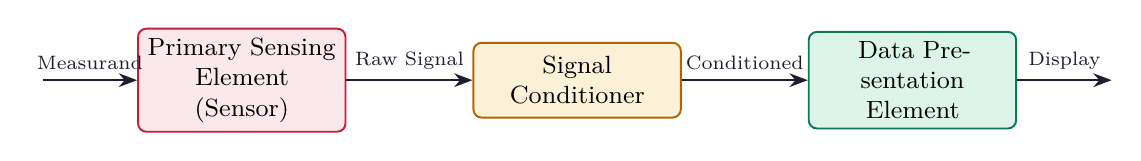
\begin{tikzpicture}[node distance=1.0cm and 1.6cm, thick, font=\small]
  \node[block, fill=hdrred, draw=myred] (sensor) {Primary Sensing\\Element (Sensor)};
  \node[block, right=1.6cm of sensor, fill=hdramber, draw=myamber] (cond) {Signal\\Conditioner};
  \node[block, right=1.6cm of cond, fill=hdrgreen, draw=mygreen] (display) {Data Presentation\\Element};

  % Path lines
  \draw[arrow] ($(sensor.west) - (1.2, 0)$) -- node[above, font=\scriptsize] {Measurand} (sensor.west);
  \draw[arrow] (sensor) -- node[above, font=\scriptsize] {Raw Signal} (cond);
  \draw[arrow] (cond) -- node[above, font=\scriptsize] {Conditioned} (display);
  \draw[arrow] (display.east) -- node[above, font=\scriptsize] {Display} ($(display.east) + (1.2, 0)$);
\end{tikzpicture}
\end{tcolorbox}

% ===============================================================================
\section{Performance Characteristics of Measuring Instruments}
% ===============================================================================

Performance parameters of any measuring device are divided into static and dynamic characteristics.

\subsection{Static Characteristics}
Static characteristics apply when the physical quantity remains constant or changes very slowly.

\begin{tcolorbox}[defbox, title={\textbf{Key Static Characteristics}}]
\begin{itemize}[leftmargin=*, itemsep=3.5pt, topsep=0pt]
  \item \textbf{Accuracy:} The closeness of an instrument reading to the true value of the measurand.
  \item \textbf{Precision:} The degree of reproducibility of measurements (scatter of readings).
  \item \textbf{Resolution:} The smallest change in the input value that can be detected by the instrument.
  \item \textbf{Sensitivity:} The ratio of the change in output deflection ($\Delta \theta_o$) to the change in input physical quantity ($\Delta q_i$): $S = \Delta \theta_o / \Delta q_i$.
  \item \textbf{Repeatability:} The closeness of agreement between successive measurements taken under identical conditions over a short time.
  \item \textbf{Reproducibility:} The consistency of readings taken by different observers, locations, or instruments over a long period.
  \item \textbf{Fidelity:} The ability of a system to reproduce the input signal without dynamic distortion.
  \item \textbf{Static Lag:} The retardation/delay in the response of an instrument to changes in the measurand.
\end{itemize}
\end{tcolorbox}

\subsection{Types of Measurement Errors}
Errors are defined as the difference between the measured value ($A_m$) and the true value ($A_t$). They are classified as:
\begin{enumerate}[label=\alph*., leftmargin=*]
  \item \textbf{Gross Errors:} Caused by human errors in reading, recording, or calculating instruments (e.g., parallax errors).
  \item \textbf{Systematic (Instrumental/Environmental/Observational) Errors:} Errors inherent in the instrument design, environment (temperature, humidity), or calibration drift. These are predictable and can be corrected.
  \item \textbf{Random Errors:} Residual errors that remain after gross and systematic errors have been eliminated. They follow a Gaussian/normal statistical distribution.
\end{enumerate}

\subsection{Dynamic Characteristics}
Dynamic characteristics apply when the input changes rapidly with time. They include:
\begin{itemize}[leftmargin=*, itemsep=2.5pt]
  \item \textbf{Speed of Response:} The rapidity with which the instrument responds to changes in the measurand.
  \item \textbf{Measuring Lag:} Delay in response to a dynamic input.
  \item \textbf{Dynamic Error:} The difference between the true value of a quantity and the value indicated by the instrument under dynamic conditions.
  \item \textbf{Fidelity:} True reproduction of dynamic inputs.
\end{itemize}

% ===============================================================================
\section{Measuring Instruments \& Range Extension}
% ===============================================================================

\subsection{D'Arsonval Movement (PMMC)}
The \textbf{Permanent Magnet Moving Coil (PMMC)} movement is the core analog indicator mechanism. It operates on the electromagnetic force principle: when current flows through a moving coil inside a magnetic field, a deflecting torque is created.
\begin{itemize}[leftmargin=*, itemsep=3.5pt]
  \item \textbf{Deflecting Torque ($T_d$):} $T_d = B \cdot A \cdot N \cdot I$ (where $B$ = flux density, $A$ = coil area, $N$ = turns, $I$ = current).
  \item \textbf{Controlling Torque ($T_c$):} Provided by hair springs: $T_c = K \cdot \theta$ (where $K$ = spring constant, $\theta$ = deflection angle).
  \item \textbf{Balance Condition:} At steady state, $T_d = T_c \implies \theta \propto I$ (linear scale).
  \item \textbf{Drawback:} Measures DC only. AC averages to zero.
\end{itemize}

\subsection{Extension of Range}
PMMC coils are delicate and can handle only small currents (typically $50\,\mu\text{A}$ to $1\,\text{mA}$). For larger ranges, multipliers and shunts are used:

\begin{tcolorbox}[formulabox, title={\textbf{Range Extension Calculations}}]
\begin{enumerate}[leftmargin=*, itemsep=4pt, label=\arabic*.]
  \item \textbf{DC Ammeter Range Extension (Shunt Resistor $R_{sh}$):}
    To measure a total current $I$ using a meter of resistance $R_m$ and full-scale current $I_m$:
    $$I_{sh} \cdot R_{sh} = I_m \cdot R_m \implies (I - I_m)R_{sh} = I_m R_m \implies R_{sh} = \frac{R_m}{\frac{I}{I_m} - 1} = \frac{R_m}{m - 1}$$
    where $m = I/I_m$ is the ammeter multiplying factor.
  \item \textbf{DC Voltmeter Range Extension (Multiplier Resistor $R_s$):}
    To measure a total voltage $V$ using a meter of resistance $R_m$ and full-scale voltage $V_m = I_m R_m$:
    $$V = I_m (R_s + R_m) \implies R_s + R_m = \frac{V}{I_m} \implies R_s = R_m \left(\frac{V}{V_m} - 1\right) = R_m(m - 1)$$
    where $m = V/V_m$ is the voltmeter multiplying factor.
\end{enumerate}
\end{tcolorbox}

\subsection{True RMS Responding Voltmeter}
Standard AC meters measure the average value and scale it by $1.11$ to indicate RMS for perfect sine waves. For non-sinusoidal waves, this causes massive errors.

\begin{itemize}[leftmargin=*, itemsep=3.5pt]
  \item \textbf{Working Principle:} True RMS voltmeters use a \textbf{thermocouple/heating element} combination. The input AC voltage is fed into a heater resistor, producing heat proportional to the RMS power ($\text{Heat} \propto V_{\text{rms}}^2$). A thermocouple converts the temperature difference into a DC voltage, driving a standard PMMC meter to indicate the true RMS value of any waveform.
\end{itemize}

% ===============================================================================
\section{Ohmmeters}
% ===============================================================================

\begin{tcolorbox}[defbox, title={\textbf{Ohmmeter}}]
An \textbf{ohmmeter} is an instrument designed to measure electrical resistance. It consists of an internal voltage source (battery), a current-limiting resistor, and a current-sensing movement (typically PMMC) that displays the resistance value on a calibrated scale.
\end{tcolorbox}

Ohmmeters are classified into two primary designs depending on how the unknown resistor $R_x$ is connected to the meter: \textbf{Series-type} and \textbf{Shunt-type}.

\subsection{Series-Type Ohmmeter}
A series-type ohmmeter connects the unknown resistor $R_x$ in series with the internal circuit. It is primarily used for measuring high resistance values (typically in the range of kilohms to megohms).

\begin{itemize}[leftmargin=*, itemsep=3.5pt]
  \item \textbf{Circuit Operation:}
    \begin{itemize}[leftmargin=*, itemsep=2.5pt, topsep=0pt]
      \item $E$: Internal battery voltage source.
      \item $R_1$: Series current-limiting resistor to protect the meter.
      \item $R_2$: Shunt zero-adjust variable resistor across the PMMC meter.
      \item $R_m$: Internal resistance of the PMMC movement.
      \item $A, B$: Connection terminals for the unknown resistor $R_x$.
    \end{itemize}
  \item \textbf{Calibration \& Zero Adjustment:}
    \begin{itemize}[leftmargin=*, itemsep=2.5pt, topsep=0pt]
      \item \textbf{Short Circuit ($R_x = 0$):} Terminals A and B are short-circuited. The total current is maximum, and the shunt resistor $R_2$ is adjusted so that the pointer deflects to its full-scale value. This Full Scale Deflection (FSD) point is marked as $0\,\Omega$ on the right side of the scale.
      \item \textbf{Open Circuit ($R_x = \infty$):} Terminals A and B are left open. The current is zero. The pointer remains at zero deflection, which is marked as $\infty\,\Omega$ on the left side of the scale.
    \end{itemize}
  \item \textbf{Scale Characteristic:} The scale is non-linear and runs from right to left ($0\,\Omega$ at FSD on the right, $\infty\,\Omega$ at zero deflection on the left). It is crowded at the high-resistance end (left).
\end{itemize}

\begin{tcolorbox}[tikzbox, title={Series-Type Ohmmeter Circuit Schematic}]
\centering
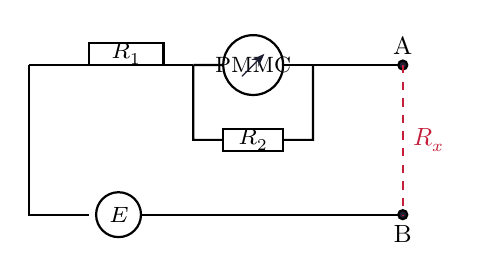
\begin{tikzpicture}[thick, scale=0.95]
  % Coordinates
  \coordinate (start) at (0,2);
  \coordinate (R1_in) at (0.8,2);
  \coordinate (R1_out) at (1.8,2);
  \coordinate (node_shunt_left) at (2.2,2);
  \coordinate (node_shunt_right) at (3.8,2);
  \coordinate (M_in) at (2.6,2);
  \coordinate (M_out) at (3.4,2);
  \coordinate (A_term) at (5.0,2);
  \coordinate (B_term) at (5.0,0);
  \coordinate (E_in) at (0,0);
  \coordinate (E_out) at (0.8,0);

  % Draw main loop
  \draw (start) -- (R1_in);
  \draw[fill=white] (R1_in) rectangle (1.8,2.3) node[midway] {\footnotesize $R_1$};
  \draw (R1_out) -- (node_shunt_left);
  \draw (node_shunt_left) -- (2.6,2);
  
  % PMMC Meter
  \draw[fill=white] (3.0,2) circle (0.4) node (M) {\footnotesize PMMC};
  \draw[arrow, thin] (2.85,1.85) -- (3.15,2.15);
  \draw (2.6,2) -- (M_in);
  \draw (M_out) -- (node_shunt_right);
  \draw (node_shunt_right) -- (A_term);
  
  % Shunt R2 path
  \draw (node_shunt_left) -- (2.2,1.0) -- (2.6,1.0);
  \draw[fill=white] (2.6,0.85) rectangle (3.4,1.15) node[midway] {\footnotesize $R_2$};
  \draw (3.4,1.0) -- (3.8,1.0) -- (node_shunt_right);
  
  % Bottom wire and Battery
  \draw (start) -- (0,0) -- (0.8,0);
  \draw[fill=white] (1.2, 0) circle (0.3) node {\footnotesize $E$};
  \draw (1.5,0) -- (B_term);
  
  % Terminals
  \draw[fill=mydark] (A_term) circle (0.06) node[above] {\small A};
  \draw[fill=mydark] (B_term) circle (0.06) node[below] {\small B};
  
  % Unknown Rx
  \draw[dashed, myred, thick] (A_term) -- (B_term) node[midway, right] {\small $R_x$};
\end{tikzpicture}
\end{tcolorbox}

\begin{tcolorbox}[formulabox, title={\textbf{Series Ohmmeter Equations}}]
The meter current $I_m$ as a function of the unknown resistance $R_x$ is:
\begin{equation}
  I_m = \frac{E \cdot R_2}{(R_x + R_1)(R_2 + R_m) + R_2 R_m}
\end{equation}
Let $R_h$ be the half-scale resistance (the value of $R_x$ when $I_m = 0.5 I_{fs}$):
\begin{equation}
  R_h = R_1 + \frac{R_2 R_m}{R_2 + R_m}
\end{equation}
The deflection ratio $s = I_m / I_{fs}$ is given by:
\begin{equation}
  s = \frac{R_h}{R_x + R_h}
\end{equation}
\end{tcolorbox}

\subsection{Shunt-Type Ohmmeter}
A shunt-type ohmmeter connects the unknown resistor $R_x$ in parallel (shunt) with the PMMC meter. It is primarily used for measuring very low resistance values (typically $1\,\Omega$ to $100\,\Omega$).

\begin{itemize}[leftmargin=*, itemsep=3.5pt]
  \item \textbf{Circuit Operation:}
    \begin{itemize}[leftmargin=*, itemsep=2.5pt, topsep=0pt]
      \item $E$: Internal battery voltage source.
      \item $R_1$: Series adjustable current-limiting resistor to calibrate the meter and limit battery drain.
      \item $S$: Switch to disconnect the battery when not in use.
      \item $R_m$: Internal resistance of the PMMC movement.
      \item $A, B$: Connection terminals for $R_x$ across the meter.
    \end{itemize}
  \item \textbf{Calibration \& Zero Adjustment:}
    \begin{itemize}[leftmargin=*, itemsep=2.5pt, topsep=0pt]
      \item \textbf{Short Circuit ($R_x = 0$):} Terminals A and B are short-circuited. No current flows through the meter ($I_m = 0$). The pointer remains at zero deflection on the left, which is marked as $0\,\Omega$.
      \item \textbf{Open Circuit ($R_x = \infty$):} Terminals A and B are open-circuited. All current flows through the meter. $R_1$ is adjusted until the meter deflects to FSD, which is marked as $\infty\,\Omega$ on the right side of the scale.
    \end{itemize}
  \item \textbf{Scale Characteristic:} The scale is non-linear and runs from left to right ($0\,\Omega$ at zero deflection on the left, $\infty\,\Omega$ at FSD on the right). It is suitable for low-value resistance measurement since low values cause measurable deflection changes near zero.
\end{itemize}

\begin{tcolorbox}[tikzbox, title={Shunt-Type Ohmmeter Circuit Schematic}]
\centering
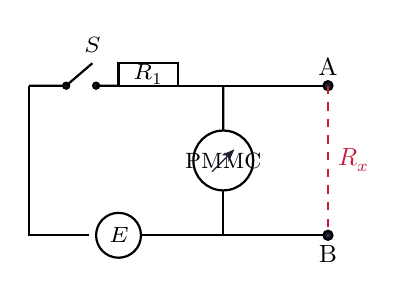
\begin{tikzpicture}[thick, scale=0.95]
  % Coordinates
  \coordinate (start) at (0,2);
  \coordinate (R1_in) at (1.2,2);
  \coordinate (R1_out) at (2.0,2);
  \coordinate (node_meter) at (2.6,2);
  \coordinate (node_term_A) at (4.0,2);
  \coordinate (E_in) at (0,0);
  \coordinate (B_term) at (4.0,0);
  
  % Draw top path with Switch
  \draw (start) -- (0.5,2);
  \draw[fill=mydark] (0.5,2) circle (0.04);
  \draw[fill=mydark] (0.9,2) circle (0.04);
  \draw (0.5,2) -- (0.85,2.3) node[above] {\footnotesize $S$};
  \draw (0.9,2) -- (R1_in);
  \draw[fill=white] (R1_in) rectangle (2.0,2.3) node[midway] {\footnotesize $R_1$};
  \draw (R1_out) -- (node_meter);
  \draw (node_meter) -- (node_term_A);
  
  % PMMC Meter branch
  \draw (node_meter) -- (2.6,1.4);
  \draw[fill=white] (2.6,1.0) circle (0.4) node {\footnotesize PMMC};
  \draw[arrow, thin] (2.45,0.85) -- (2.75,1.15);
  \draw (2.6,0.6) -- (2.6,0);
  
  % Battery
  \draw (start) -- (0,0) -- (0.8,0);
  \draw[fill=white] (1.2, 0) circle (0.3) node {\footnotesize $E$};
  \draw (1.5,0) -- (B_term);
  
  % Connections at bottom
  \draw (2.6,0) -- (B_term);
  
  % Terminals
  \draw[fill=mydark] (node_term_A) circle (0.06) node[above] {\small A};
  \draw[fill=mydark] (B_term) circle (0.06) node[below] {\small B};
  
  % Unknown Rx
  \draw[dashed, myred, thick] (node_term_A) -- (B_term) node[midway, right] {\small $R_x$};
\end{tikzpicture}
\end{tcolorbox}

\begin{tcolorbox}[formulabox, title={\textbf{Shunt Ohmmeter Equations}}]
The meter current $I_m$ is given by:
\begin{equation}
  I_m = \frac{E R_x}{R_1(R_x + R_m) + R_x R_m}
\end{equation}
When $R_1 \gg R_m$, we can simplify to:
\begin{equation}
  I_m \approx \frac{E}{R_1} \left( \frac{R_x}{R_x + R_m} \right)
\end{equation}
The half-scale resistance $R_h$ where $I_m = 0.5 I_{fs}$ is approximately:
\begin{equation}
  R_h = \frac{R_1 R_m}{R_1 + R_m} \approx R_m
\end{equation}
The deflection ratio $s = I_m / I_{fs}$ is:
\begin{equation}
  s = \frac{R_x}{R_x + R_h}
\end{equation}
\end{tcolorbox}

% ===============================================================================
\section{Multimeters}
% ===============================================================================

\begin{tcolorbox}[defbox, title={\textbf{Multimeter}}]
A \textbf{multimeter} is a multi-purpose electronic measuring instrument that integrates several measurement functions---typically voltage, current, and resistance---into a single device.
\end{tcolorbox}

Multimeters are available in two forms: \textbf{Analog Multimeters} (often called VOM) and \textbf{Digital Multimeters} (DMM).

\subsection{Analog Multimeter (VOM)}
An Analog Multimeter (Volt-Ohm-Milliammeter or VOM) uses a standard PMMC movement as the central indicator. A multi-deck, multi-position rotary selector switch connects different internal networks to the meter.

\begin{itemize}[leftmargin=*, itemsep=3.5pt]
  \item \textbf{Sub-circuits \& Function Selection:}
    \begin{itemize}[leftmargin=*, itemsep=2.5pt, topsep=0pt]
      \item \textbf{DC Voltage:} Extends range using series multiplier resistors.
      \item \textbf{AC Voltage:} Uses a diode rectifier network (half-wave or full-wave) to convert AC to DC, which is then scaled by series multipliers.
      \item \textbf{DC Current:} Extends range using parallel shunt resistors.
      \item \textbf{Resistance:} Uses an internal battery and calibrating resistors configured as series or shunt ohmmeters.
    \end{itemize}
  \item \textbf{Sensitivity:} Voltmeter sensitivity is expressed in ohms-per-volt ($\Omega/\text{V}$), equal to $1 / I_{fs}$. A typical VOM has a DC sensitivity of $20\,\text{k}\Omega/\text{V}$.
\end{itemize}

\begin{tcolorbox}[tikzbox, title={Analog Multimeter (VOM) Block Schematic}]
\centering
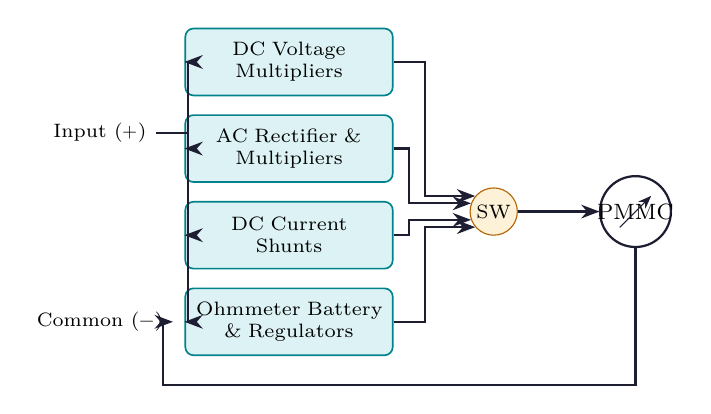
\begin{tikzpicture}[font=\small, >=Stealth,
  sblock/.style={rectangle, draw=myteal, fill=hdrteal, text width=2.4cm,
    align=center, minimum height=0.85cm, font=\scriptsize,
    rounded corners=3pt, line width=0.6pt}]
  
  % Input terminals on left
  \node (input) at (0, 1.8) {\scriptsize Input ($+$)};
  \node (common) at (0, -0.6) {\scriptsize Common ($-$)};

  % Blocks positioned with clear vertical separation
  \node[sblock] (dcv) at (2.4, 2.7) {DC Voltage\\Multipliers};
  \node[sblock] (acv) at (2.4, 1.6) {AC Rectifier \&\\Multipliers};
  \node[sblock] (dci) at (2.4, 0.5) {DC Current\\Shunts};
  \node[sblock] (ohm) at (2.4, -0.6) {Ohmmeter Battery\\\& Regulators};

  % Selector Switch
  \node[circle, draw=myamber, fill=hdramber, minimum size=0.6cm, inner sep=0pt] (sw) at (5.0, 0.8) {\scriptsize SW};

  % PMMC Meter
  \node[circle, draw=mydark, fill=white, minimum size=0.9cm] (pmmc) at (6.8, 0.8) {};
  \draw[thick, color=mydark] (pmmc.center) circle (0.45);
  \node at (pmmc.center) {\footnotesize PMMC};
  \draw[arrow, thin] ($(pmmc.center)+(-0.2,-0.2)$) -- ($(pmmc.center)+(0.2,0.2)$);

  % Connections from Input to Blocks
  \draw[arrow] (input.east) -- ++(0.4, 0) |- (dcv.west);
  \draw[arrow] (input.east) -- ++(0.4, 0) |- (acv.west);
  \draw[arrow] (input.east) -- ++(0.4, 0) |- (dci.west);
  \draw[arrow] (input.east) -- ++(0.4, 0) |- (ohm.west);

  % Connections from Blocks to Selector Switch (SW)
  \draw[arrow] (dcv.east) -- ++(0.4, 0) |- (sw.140);
  \draw[arrow] (acv.east) -- ++(0.2, 0) |- (sw.160);
  \draw[arrow] (dci.east) -- ++(0.2, 0) |- (sw.200);
  \draw[arrow] (ohm.east) -- ++(0.4, 0) |- (sw.220);

  % Switch to PMMC
  \draw[arrow] (sw.east) -- (pmmc.west);

  % PMMC Return to Common (completely clear of all blocks, going below the bottom block)
  \draw[arrow] (pmmc.south) -- (6.8, -1.4) -- (0.8, -1.4) |- (common.east);
\end{tikzpicture}
\end{tcolorbox}

\subsection{Digital Multimeter (DMM)}
A Digital Multimeter (DMM) processes signals electronically and displays the measured values numerically. DMMs offer higher accuracy, higher input impedance ($10\,\text{M}\Omega$ to eliminate loading effects), and auto-ranging capabilities.

\begin{itemize}[leftmargin=*, itemsep=3.5pt]
  \item \textbf{Signal Conditioning Stages:}
    \begin{itemize}[leftmargin=*, itemsep=2.5pt, topsep=0pt]
      \item \textbf{AC Voltage:} Scale down by an attenuator and convert to DC using an active precision rectifier.
      \item \textbf{DC Current:} Force the current through low-resistance shunts and measure the resulting voltage drop.
      \item \textbf{Resistance:} Pass a constant current from an internal source through the unknown resistor $R_x$ to generate a voltage drop ($V_x = I_{\text{const}} \cdot R_x$).
    \end{itemize}
  \item \textbf{Dual-Slope Integration ADC:} DMMs use a Dual-Slope ADC for converting analog voltages into digital form due to its superior noise rejection.
\end{itemize}

\begin{tcolorbox}[tikzbox, title={Digital Multimeter (DMM) Block Diagram}]
\centering
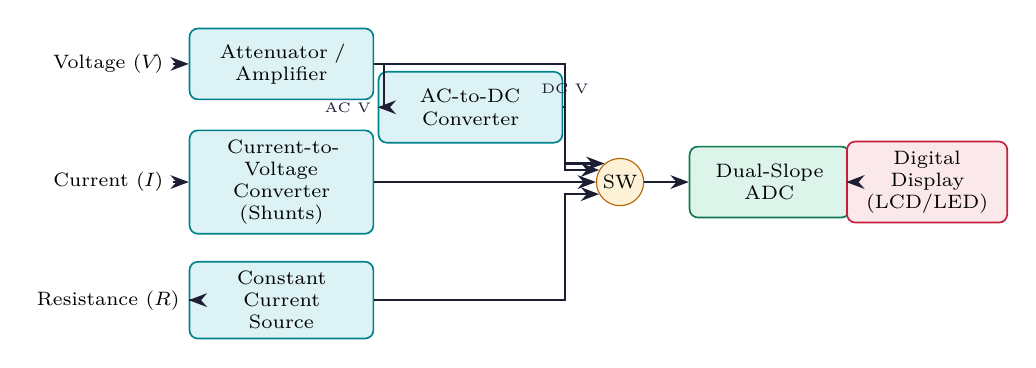
\begin{tikzpicture}[font=\small, >=Stealth,
  sblock/.style={rectangle, draw=myteal, fill=hdrteal, text width=2.1cm,
    align=center, minimum height=0.9cm, font=\scriptsize,
    rounded corners=3pt, line width=0.6pt}]
  
  % Inputs on the left
  \node (in_v) at (0, 2.4) {\scriptsize Voltage ($V$)};
  \node (in_i) at (0, 0.9) {\scriptsize Current ($I$)};
  \node (in_r) at (0, -0.6) {\scriptsize Resistance ($R$)};
  
  % First-stage blocks
  \node[sblock] (attn) at (2.2, 2.4) {Attenuator /\\Amplifier};
  \node[sblock] (shunt) at (2.2, 0.9) {Current-to-Voltage\\Converter (Shunts)};
  \node[sblock] (const_i) at (2.2, -0.6) {Constant Current\\Source};
  
  % AC-to-DC Converter (lowered for clear branching)
  \node[sblock] (rect) at (4.6, 1.85) {AC-to-DC\\Converter};
  
  % Selector Switch (SW)
  \node[circle, draw=myamber, fill=hdramber, minimum size=0.6cm, inner sep=0pt] (sw) at (6.5, 0.9) {\scriptsize SW};
  
  % ADC & Display
  \node[sblock, fill=hdrgreen, draw=mygreen, text width=1.8cm] (adc) at (8.4, 0.9) {Dual-Slope\\ADC};
  \node[sblock, fill=hdrred, draw=myred, text width=1.8cm] (disp) at (10.4, 0.9) {Digital Display\\(LCD/LED)};
  
  % Connections
  % Voltage path
  \draw[arrow] (in_v) -- (attn);
  \draw[line] (attn.east) -- (3.5, 2.4) coordinate (v_split);
  \draw[arrow] (v_split) -- (5.8, 2.4) |- (sw.130) node[pos=0.2, above, font=\tiny] {DC V};
  \draw[arrow] (v_split) |- (rect.west) node[pos=0.7, left, font=\tiny] {AC V};
  \draw[arrow] (rect.east) -- (5.8, 1.85) |- (sw.150);
  
  % Current path
  \draw[arrow] (in_i) -- (shunt);
  \draw[arrow] (shunt.east) -- (sw.180);
  
  % Resistance path
  \draw[arrow] (in_r) -- (const_i);
  \draw[arrow] (const_i.east) -- (5.8, -0.6) |- (sw.210);
  
  % Switch to ADC and Display
  \draw[arrow] (sw.east) -- (adc.west);
  \draw[arrow] (adc.east) -- (disp.west);
\end{tikzpicture}
\tcbset{breakable}
\end{tcolorbox}

\begin{tcolorbox}[formulabox, title={\textbf{Dual-Slope ADC Integration Principle}}]
The Dual-Slope ADC operates in two phases:
\begin{enumerate}[leftmargin=*, itemsep=2.5pt]
  \item \textbf{Integrate Phase (Fixed Time $T_1$):} The input voltage $V_{\text{in}}$ is integrated for a predetermined fixed duration $T_1 = 2^N \cdot T_{\text{clk}}$. The integrator output voltage rises to:
    \begin{equation}
      V_p = -\frac{V_{\text{in}}}{RC} T_1
    \end{equation}
  \item \textbf{De-integrate Phase (Variable Time $T_2$):} A reference voltage $-V_{\text{ref}}$ of opposite polarity is connected to the integrator. The output ramps down to zero at a constant rate. The variable time $T_2$ taken to return to zero is measured by counting clock pulses:
    \begin{equation}
      V_p = \frac{V_{\text{ref}}}{RC} T_2
    \end{equation}
\end{enumerate}
Equating the two peak values, we obtain the voltage relationship:
\begin{equation}
  V_{\text{in}} = V_{\text{ref}} \left( \frac{T_2}{T_1} \right)
\end{equation}
\textbf{Key Advantage:} The measurement depends only on the ratio of times $T_2/T_1$ and $V_{\text{ref}}$, completely eliminating errors due to component tolerances/aging of $R$ and $C$ or clock frequency drift.
\end{tcolorbox}

\newpage
% ===============================================================================
% MANDATORY QUICK REVISION PAGE
% ===============================================================================
\begin{center}
  {\large\bfseries\color{myred} Quick Revision --- Module 1}\\[3pt]
  {\small\color{mydark} Block Schematics \& Basic Instruments $|$ OE-EC604A}
\end{center}
\noindent{\color{myred}\rule{\linewidth}{1.2pt}}
\vspace{4pt}

\begin{tcolorbox}[formulabox, title={\textbf{Key Formulas at a Glance}}]
\begin{align*}
  \text{Ammeter Shunt:} \quad & R_{sh} = \frac{R_m}{m - 1} \quad \text{where} \ m = \frac{I}{I_m} \\
  \text{Voltmeter Multiplier:} \quad & R_s = R_m(m - 1) \quad \text{where} \ m = \frac{V}{V_m} \\
  \text{Series Ohmmeter Deflection:} \quad & s = \frac{I_m}{I_{fs}} = \frac{R_h}{R_x + R_h} \quad \text{where} \ R_h = R_1 + R_2 \parallel R_m \\
  \text{Shunt Ohmmeter Deflection:} \quad & s = \frac{I_m}{I_{fs}} = \frac{R_x}{R_x + R_h} \quad \text{where} \ R_h = R_1 \parallel R_m \approx R_m \\
  \text{DMM Dual-Slope ADC:} \quad & V_{\text{in}} = V_{\text{ref}} \left(\frac{T_2}{T_1}\right)
\end{align*}
\end{tcolorbox}

\begin{tcolorbox}[defbox, title={\textbf{One-Line Definitions}}]
\begin{itemize}[leftmargin=*, itemsep=2.5pt, topsep=0pt]
  \item \textbf{Accuracy:} Degree of closeness of a measured value to the actual true value.
  \item \textbf{Precision:} Degree of agreement/repeatability within a group of measurements.
  \item \textbf{Resolution:} The smallest detectable change in the input measurand.
  \item \textbf{PMMC:} Permanent Magnet Moving Coil movement; sensitive DC indicator based on magnetic coil torque.
  \item \textbf{True RMS Voltmeter:} Instrument measuring heating power of input signal to compute exact RMS regardless of shape.
  \item \textbf{Series-type Ohmmeter:} Ohmmeter where the unknown resistance is in series with the meter; zero is on the right of the scale.
  \item \textbf{Shunt-type Ohmmeter:} Ohmmeter where the unknown resistance is in parallel with the meter; zero is on the left of the scale.
  \item \textbf{Dual-Slope ADC:} An analog-to-digital converter that integrates input voltage and then de-integrates reference voltage, rejecting noise.
\end{itemize}
\end{tcolorbox}

\begin{tcolorbox}[exambox, title={\textbf{Frequently Asked / Viva Questions}}]
\begin{enumerate}[topsep=0pt, label=\textbf{Q\arabic*.}, itemsep=5pt]
  \item \Q{Differentiate between Accuracy and Precision.}
    Accuracy is the closeness of a measured value to the true value, whereas precision is the repeatability of readings when measured repeatedly. An instrument can be highly precise but inaccurate if it has a constant offset error.
  \item \Q{A PMMC meter has internal resistance $R_m = 100\,\Omega$ and full-scale deflection current $I_m = 1\,\text{mA}$. Calculate the shunt resistance required to extend its range to $1\,\text{A}$.}\\
    Given: $R_m = 100\,\Omega$, $I_m = 1\,\text{mA} = 0.001\,\text{A}$, Target current $I = 1\,\text{A}$.\par
    Multiplying factor: $m = I / I_m = 1 / 0.001 = 1000$.\par
    Shunt resistance: $R_{sh} = R_m / (m - 1) = 100 / (1000 - 1) = 100 / 999 \approx 0.1001\,\Omega$.
  \item \Q{Using the same PMMC meter ($R_m=100\,\Omega, I_m=1\,\text{mA}$), calculate the multiplier resistance required to extend its range to measure a voltmeter scale of $100\,\text{V}$.}\\
    Full scale meter voltage: $V_m = I_m \cdot R_m = 0.001 \times 100 = 0.1\,\text{V}$.\par
    Multiplying factor: $m = V / V_m = 100 / 0.1 = 1000$.\par
    Multiplier series resistance: $R_s = R_m(m - 1) = 100 \times 999 = 99,900\,\Omega = 99.9\,\text{k}\Omega$.
  \item \Q{Why does a PMMC instrument fail to measure AC values directly?}
    Because the direction of deflecting torque depends on the current polarity. For AC, the current alternates polarity rapidly (e.g., $50\,\text{Hz}$). The pointer attempts to follow the oscillations but due to inertia, it stays at zero, displaying only the average value (which is 0 for AC).
  \item \Q{What is True RMS and why is it preferred over average-responding voltmeters?}
    Average-responding voltmeters rectify AC, find the average, and multiply it by $1.11$ (the form factor for a sine wave) to display RMS. This is invalid for square, triangular, or distorted waves. A True RMS voltmeter measures the actual thermal power generated by the signal, representing its true heating equivalent.
  \item \Q{Compare Series and Shunt type Ohmmeters.}
    In a series ohmmeter, the unknown resistor $R_x$ is in series with the PMMC meter. Zero resistance ($0\,\Omega$) corresponds to full-scale deflection (FSD) on the right. In a shunt ohmmeter, $R_x$ is in parallel with the meter. Zero resistance ($0\,\Omega$) corresponds to zero deflection on the left.
  \item \Q{What is the main advantage of a Digital Multimeter (DMM) over an analog VOM?}
    A DMM provides high input impedance (typically $10\,\text{M}\Omega$ across all ranges), which prevents loading errors. It also offers digital numerical displays (no parallax errors), auto-ranging, and greater accuracy.
  \item \Q{Explain why a Dual-Slope ADC is preferred in DMMs.}
    It has excellent noise rejection (particularly line frequency noise like $50\,\text{Hz}$/ $60\,\text{Hz}$ if integration time is chosen as a multiple of the line period). Additionally, the conversion accuracy is independent of the values of the integrating capacitor and resistor, and the clock frequency.
  \item \Q{What are systematic errors and how can they be minimized?}
    Systematic errors are predictable, constant errors arising from instrument calibration, component aging, or environmental changes (temperature/humidity). They can be minimized by periodic calibration, proper shielding, and applying mathematical correction factors.
  \item \Q{What is static lag and how does it differ from dynamic lag?}
    Static lag is the delay in response when the input measurand is constant or changing very slowly, caused by friction or spring inertia. Dynamic lag occurs when the input changes rapidly, caused by the system's dynamic parameters (mass, damping, capacitance).
\end{enumerate}
\end{tcolorbox}

\begin{tcolorbox}[tikzbox, title={Accuracy vs Precision Comparison Summary}]
\renewcommand{\arraystretch}{1.4}
\par\noindent
\begin{tabularx}{\linewidth}{|B{2.2cm}|>{\small\centering\arraybackslash}X|>{\small\centering\arraybackslash}X|}
\hline
\textbf{Feature} & \textbf{\color{myred}Accuracy} & \textbf{\color{myteal}Precision} \\
\hline
\textbf{Core Concept} & Closeness to the actual true value. & Closeness of multiple readings to each other. \\
\hline
\textbf{Error Type} & Linked to systematic errors. & Linked to random errors (scatter). \\
\hline
\textbf{Calibration} & Can be improved by calibration. & Calibration does not improve precision. \\
\hline
\textbf{Dependence} & Requires precision to be accurate. & Can be highly precise but inaccurate. \\
\hline
\textbf{Time Period} & Measured over short term. & Represents stability over short term. \\
\hline
\end{tabularx}
\end{tcolorbox}


\end{document}
